\documentclass[a4paper]{article}
\usepackage[utf8]{inputenc}
\usepackage[spanish, es-tabla, es-noshorthands]{babel}
\usepackage[table,xcdraw]{xcolor}
\usepackage[a4paper, footnotesep = 1cm, width=20cm, top=2.5cm, height=25cm, textwidth=18cm, textheight=25cm]{geometry}
%\geometry{showframe}

\usepackage{tikz}
\usepackage{amsmath}
\usepackage{amsfonts}
\usepackage{amssymb}
\usepackage{float}
\usepackage{graphicx}
\usepackage{caption}
\usepackage{subcaption}
\usepackage{multicol}
\usepackage{multirow}
\setlength{\doublerulesep}{\arrayrulewidth}
\usepackage{booktabs}

\usepackage{hyperref}
\hypersetup{
    colorlinks=true,
    linkcolor=blue,
    filecolor=magenta,      
    urlcolor=blue,
    citecolor=blue,    
}

\newcommand{\quotes}[1]{``#1''}
\usepackage{array}
\newcolumntype{C}[1]{>{\centering\let\newline\\\arraybackslash\hspace{0pt}}m{#1}}
\usepackage[american]{circuitikz}
\usetikzlibrary{calc}
\usepackage{fancyhdr}
\usepackage{units} 

\graphicspath{{../Ejercicio-1/}{../Ejercicio-2/}{../Ejercicio-3/}{../Ejercicio-4/}}

\pagestyle{fancy}
\fancyhf{}
\lhead{22.01 Teoría de Circuitos}
\rhead{Mechoulam, Lambertucci, Rodriguez Turco, Londero, Galdeman}
\rfoot{\centering \thepage}
\begin{document}

\subsection{Introducción}

En esta sección se implementó un filtro Band-Pass utilizando una aproximación \textbf{Chebycheff} e implementandola con celdas \textbf{Rauch}, el filtro a diseñar deberá cumplir con la siguiente plantilla.
\begin{table}[H]
\centering
\begin{tabular}{|c|c|}
\hline
$Pendiente$      & -40$\frac{dB}{dec}$           \\ \hline
$f_p$      & 28kHz          \\ \hline
$B$      & $\frac{1}{10}$           \\ \hline
$A_p$      & 3dB               \\ \hline
$Filtro$      & BP              \\ \hline
$|Z_{in}|$ & $\geq 50k \Omega$ \\ \hline
\end{tabular}
\end{table}
\subsection{Aproximación de Chebycheff.}
Para esta sección se utlizó la aproximación de \textbf{Chebyfeff}, además se propuso una plantilla mas restrictiva, con el fin de asegurar el cumplimiento de la original. 

Se despejó el valor de $f_p^+$ y $f_p^-$ 
\begin{align}
f_0^2 = f_p^+ \cdot f_p^- \\
B = \frac{\Delta f_p}{f_0}\\
f_p^+ =29.435 kHz  \ \ \ f_p^- = 26.635 kHz
\end{align}
Luego teniendo en cuenta que la pendiente originalmente es de 40dB por decada se tomo la frecuencia de atenuación acorde  talque mantenga las condiciones de simetría, siendo estas: $f_a^+= 294.35kHz y f_a^- = 2.635kHz$.


Siendo esta la plantilla final.
\begin{table}[H]
\centering
\begin{tabular}{|c|c|}
\hline
$f_s^-$      & 2.2635 kHz          \\ \hline
$f_p^-$      & 26.635 kHz         \\ \hline
$f_p^+$      & 29.435 kHz           \\ \hline
$f_s^+$      & 304.35 kHz          \\ \hline
$A_s$      & 40dB           \\ \hline
$A_p$      & 1dB               \\ \hline
\end{tabular}
\end{table}
Obteniendo la siguiente función transferencia:
\begin{align}
	H(s)=\frac{s\cdot -1.0448\cdot 10^{5}}{s^2+s\cdot 71653+5.2722\cdot 10^{10}}\cdot \frac{s \cdot -74995}{s^2+s\cdot 51101+2.7236 \cdot 10^{10}}
\end{align}
al cual le corresponde la siguiente respues en frecuencia:

Y el siguiente diagrama de polos y ceros:
\begin{figure}[H]
	\centering
	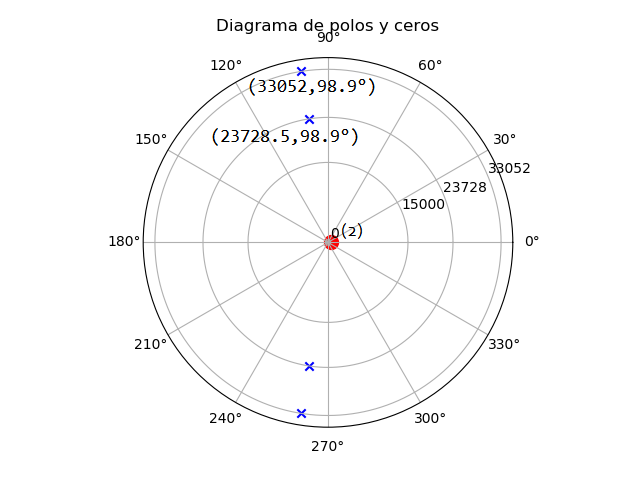
\includegraphics[width=0.5\textwidth]{Imagenes-Ej2/DiagramaPolosYCeros.png}
	\label{fig:stepresponse}
	\caption{Diagrama Polos y Ceros}
\end{figure}

Teniendo los pares de polos conjugados un Q de 3.23	


\subsubsection{Elecciones de diseño}
Se decidió armar etapas con celdas segundo orden en cascada dado a que el orden es 4.
Para la asociación de polos se tomo criterio agrupar cada par de polos con 1 cero , agrupandolos de las siguiente forma.
\begin{figure}[H]
	\centering
	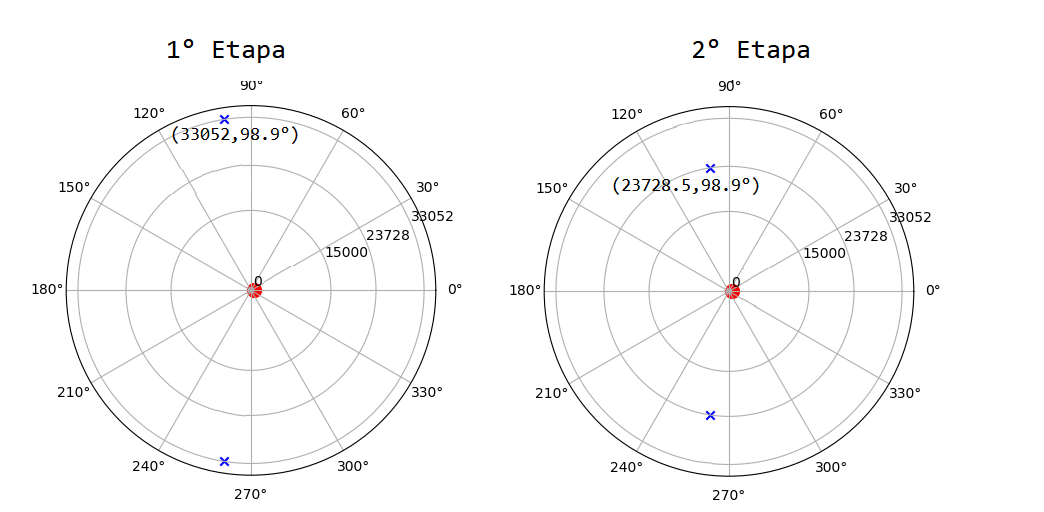
\includegraphics[width=\textwidth]{Imagenes-Ej2/UnionCeros.png}
	\label{fig:CeroPoleUnion}
	\caption{Diagrama Polos y Ceros para cada etapa}
\end{figure}

\subsection{Celda Rauch.}
\subsubsection{Cálculo Analítico.}
El circuito clásico para una celda 	Rauch pasa-banda (Deliyannis-Friend) es el siguiente:
\begin{figure}[H]
	\centering
	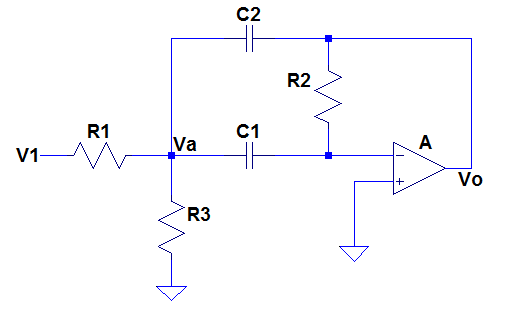
\includegraphics[width=0.5\textwidth]{Imagenes-Ej2/rauchoriginal.PNG}
	\label{fig:graph}
	\caption{Circuito clásico celda Rauch Band-Pass(Deliyannis-Friend) .}
\end{figure}
De aquí, planteando los nodos y considerando el amplificador operacional ideal se pueden hallar las siguientes ecuaciones:
\begin{align}
\frac{V_{out}}{R_2}=-V_a\cdot sC_1\\ 
\frac{V_{in}-V_a}{R_1}+(V_{out}-V_a)\cdot sC_2 -V_a \cdot sC_1 = \frac{V_a}{R_3}
\end{align}
De aqui se puede despejar la función transferencia como:
\begin{align}
H(s)=\frac{s \cdot C_1R_2R_3}{s^2\cdot R_1R_2C_2C_1+s\cdot (C_3R_1R_3+R_1C_2R_3)+R_3+R_1}=\frac{H_0 \cdot \frac{s}{\omega_0 Q}}{\frac{s^2}{\omega_0^2}+\frac{s}{\omega_0Q}+1}
\end{align}

De aquí se pueden extraer los parámetros típicos del diseño de filtros siendo los siguientes:
\begin{align}
H_0 =\frac{R_2C_2}{R_1C_2+C_1R_1}\\
\omega_0^2= \frac{R_1+R_3}{R_1^2R_2C_2C_1}\\
Q= \frac{\sqrt[]{1+\frac{R_3}{R_1}}}{{\sqrt[]{\frac{R_3C_1}{R_2C_2}}+\sqrt[]{\frac{R_3C_2}{R_2C_1}}}}
\end{align}
Luego para hacer facil la elección de componentes se suele tomar $C_1 \ = \ C_2$, por culpa de esto para obtener un Q relativamente alto se necesitan valore s de resistencia altos, lo cual es un problema.
Para solucionar dicho problema se hizo una modificación a la celda, incluyendo una realimentación positiva, permitiendo obtener un Q de mayor valor.
La celda Rauch con Q mejorado le corresponde el siguiente circuito.
\begin{figure}[H]
	\centering
	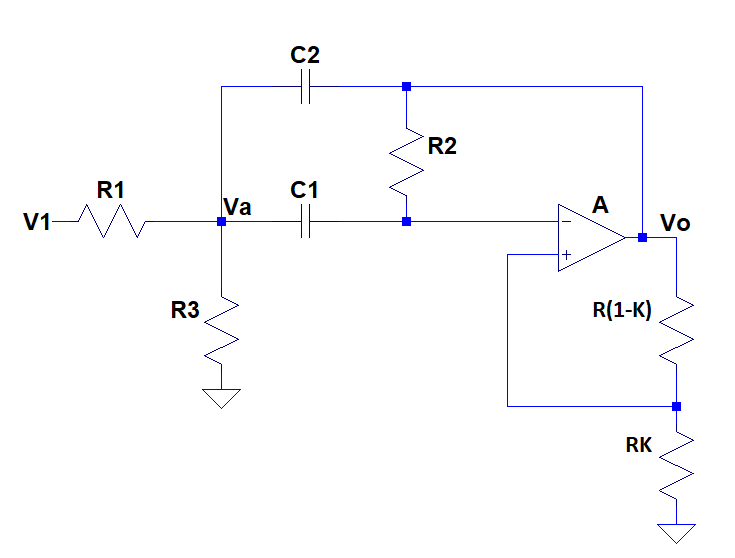
\includegraphics[width=0.5\textwidth]{Imagenes-Ej2/Circuit.PNG}
	\label{fig:graph}
	\caption{Circuito celda Rauch Band-Pass con Q enhancmente.}
\end{figure}
para resolver el circuito basta con plantear los siguientes nodos:
\begin{align}
\frac{V_{out}-K \cdot V_{out}}{R_2}=(K \cdot V_{out}-V_a)\cdot sC_1\\ 
\frac{V_{in}-V_a}{R_1}+(V_{out}-V_a)\cdot sC_2 +(K \cdot V_{out}-V_a) \cdot sC_1 = \frac{V_a}{R_3}
\end{align}
Resolviendo la transferencia se llega a la siguiente expresión:
\begin{align}
H(s)=\frac{1}{1-K} \cdot \frac{H_0 \cdot \frac{s}{\omega_0 Q_0}}{\frac{s^2}{\omega_0^2}+\frac{s}{\omega_0Q}+1}
\end{align}
Donde $Q_0$ es una constante de valor 1.5\footnote{[1]R. Schaumann, H. Xiao, M. Van Valkenburg, M. Van Valkenburg and M. Van Valkenburg, Analog filter design. New York: Oxford University Press, 2011, pp. 170-176.}, y el K es utilizado para ajustar el valor de Q del circuito, dado que quedarán así definidos los parámetros del filtro:
\begin{align}
\omega_0^2= \frac{R_1+R_3}{R_1R_3R_2C_2C_1}
\label{eq:omeg}
\end{align}
\begin{align}
Q=\frac{Q_0}{1-2Q_0^2\cdot \frac{K}{1-K}}=\frac{\sqrt[]{R_1R_3R_2C_1C_2(R_1+R_3)}}{R_1R_3(C_1+C_2)-\frac{K}{1-K}(R_1+R_3)R_2C_1}
\label{eq:Q}
\end{align}
\begin{align}
H_0=\frac{R_3R_2}{(C_1+C_2)\cdot (K-1)R_1R_3+K(R_1+R_3)R_2 C_2}
\label{eq:H0}
\end{align}
También es posible despejar la impedancia de entrada de la celda.
\begin{align}
Z_{in}(s)=\frac{V_{in}(s)}{I_{in}(s)}= \frac{s^2 R_1R_2R_3C_1C_2+s\cdot R_1R_3(C_1+C_2)+R_1+R_3}{s^2R_3R_2C_1C_2+sR_3(C_1+C_2)+1}
\end{align}
\subsubsection{Elecciones de diseño}
Realizando el cálculo de sensibilidades a partir de las expresiones (\ref{eq:omeg}) (\ref{eq:H0}) y (\ref{eq:Q}) bajo la siguiente definición:
\begin{align}
S_x^{f(x)}= \frac{\partial f(x)}{\partial x}\cdot \frac{x}{f(x)}
\end{align}
Obteniendo las siguientes tablas.

\begin{table}[H]
\centering
\begin{tabular}{ccc}
Componente & $S^{\omega_0}$ & $S^{H_0}$ \\ \cline{1-3}\\
$S_{R_1}$  & $-{\frac {{\it R3}}{ 2.0\,{\it R1}+ 2.0\,{\it R3}}}$    &$ -{\frac { \left( {\it C1}\,K{\it R3}+K{\it R2}\,{\it C2}+{\it C2}\,K{
\it R3}-{\it C1}\,{\it R3}-{\it C2}\,{\it R3} \right) {\it R1}}{{\it 
C1}\,K{\it R1}\,{\it R3}+K{\it R2}\,{\it C2}\,{\it R1}+{\it C2}\,K{
\it R1}\,{\it R3}+K{\it R2}\,{\it C2}\,{\it R3}-{\it C1}\,{\it R1}\,{
\it R3}-{\it C2}\,{\it R1}\,{\it R3}}} $  \\
$S_{R_2}$  & -0.5    & ${\frac {{\it R1}\,{\it R3}\, \left( {\it C1}\,K+{\it C2}\,K-{\it C1}-{
\it C2} \right) }{{\it C1}\,K{\it R1}\,{\it R3}+K{\it R2}\,{\it C2}\,{
\it R1}+{\it C2}\,K{\it R1}\,{\it R3}+K{\it R2}\,{\it C2}\,{\it R3}-{
\it C1}\,{\it R1}\,{\it R3}-{\it C2}\,{\it R1}\,{\it R3}}}$   \\
$S_{R_3}$  & $-{\frac {{\it R1}}{ 2.0\,{\it R1}+ 2.0\,{\it R3}}}$     & ${\frac {K{\it R2}\,{\it C2}\,{\it R1}}{{\it C1}\,K{\it R1}\,{\it R3}+K
{\it R2}\,{\it C2}\,{\it R1}+{\it C2}\,K{\it R1}\,{\it R3}+K{\it R2}\,
{\it C2}\,{\it R3}-{\it C1}\,{\it R1}\,{\it R3}-{\it C2}\,{\it R1}\,{
\it R3}}}$   \\
$S_{C_1}$  & -0.5    & $-{\frac {{\it R3}\,{\it R1}\, \left( -1+K \right) {\it C1}}{{\it C1}\,
K{\it R1}\,{\it R3}+K{\it R2}\,{\it C2}\,{\it R1}+{\it C2}\,K{\it R1}
\,{\it R3}+K{\it R2}\,{\it C2}\,{\it R3}-{\it C1}\,{\it R1}\,{\it R3}-
{\it C2}\,{\it R1}\,{\it R3}}}$  \\
$S_{C_2}$  & -0.5    & $-{\frac { \left( K{\it R2}\,{\it R1}+{\it R1}\,{\it R3}\,K+K{\it R2}\,
{\it R3}-{\it R1}\,{\it R3} \right) {\it C2}}{{\it C1}\,K{\it R1}\,{
\it R3}+K{\it R2}\,{\it C2}\,{\it R1}+{\it C2}\,K{\it R1}\,{\it R3}+K{
\it R2}\,{\it C2}\,{\it R3}-{\it C1}\,{\it R1}\,{\it R3}-{\it C2}\,{
\it R1}\,{\it R3}}}$ 
\end{tabular}
\caption{Tabla de sensibilidades $\omega_0$ y Ganancia.}
\end{table}
\begin{table}[H]
\centering
\begin{tabular}{cc}
Componente & $S^{Q}$ \\ \hline\\
$S_{R_1}$  & $1/2\,{\frac {{\it R3}\, \left( K{\it R2}\,{\it C1}\,{\it R1}-{\it C1}
\,K{\it R1}\,{\it R3}+K{\it R2}\,{\it C1}\,{\it R3}-{\it C2}\,K{\it R1
}\,{\it R3}+{\it C1}\,{\it R1}\,{\it R3}+{\it C2}\,{\it R1}\,{\it R3}
 \right) }{ \left( K{\it R2}\,{\it C1}\,{\it R1}+{\it C1}\,K{\it R1}\,
{\it R3}+K{\it R2}\,{\it C1}\,{\it R3}+{\it C2}\,K{\it R1}\,{\it R3}-{
\it C1}\,{\it R1}\,{\it R3}-{\it C2}\,{\it R1}\,{\it R3} \right) 
 \left( {\it R1}+{\it R3} \right) }}$ \\
$S_{R_2}$  & $-1/2\,{\frac {K{\it R2}\,{\it C1}\,{\it R1}-{\it C1}\,K{\it R1}\,{\it 
R3}+K{\it R2}\,{\it C1}\,{\it R3}-{\it C2}\,K{\it R1}\,{\it R3}+{\it 
C1}\,{\it R1}\,{\it R3}+{\it C2}\,{\it R1}\,{\it R3}}{K{\it R2}\,{\it 
C1}\,{\it R1}+{\it C1}\,K{\it R1}\,{\it R3}+K{\it R2}\,{\it C1}\,{\it 
R3}+{\it C2}\,K{\it R1}\,{\it R3}-{\it C1}\,{\it R1}\,{\it R3}-{\it C2
}\,{\it R1}\,{\it R3}}}$ \\
$S_{R_3}$  & $1/2\,{\frac {{\it R1}\, \left( K{\it R2}\,{\it C1}\,{\it R1}-{\it C1}
\,K{\it R1}\,{\it R3}+K{\it R2}\,{\it C1}\,{\it R3}-{\it C2}\,K{\it R1
}\,{\it R3}+{\it C1}\,{\it R1}\,{\it R3}+{\it C2}\,{\it R1}\,{\it R3}
 \right) }{ \left( K{\it R2}\,{\it C1}\,{\it R1}+{\it C1}\,K{\it R1}\,
{\it R3}+K{\it R2}\,{\it C1}\,{\it R3}+{\it C2}\,K{\it R1}\,{\it R3}-{
\it C1}\,{\it R1}\,{\it R3}-{\it C2}\,{\it R1}\,{\it R3} \right) 
 \left( {\it R1}+{\it R3} \right) }}$ \\
$S_{C_1}$  & $-1/2\,{\frac {K{\it R2}\,{\it C1}\,{\it R1}+{\it C1}\,K{\it R1}\,{\it 
R3}+K{\it R2}\,{\it C1}\,{\it R3}-{\it C2}\,K{\it R1}\,{\it R3}-{\it 
C1}\,{\it R1}\,{\it R3}+{\it C2}\,{\it R1}\,{\it R3}}{K{\it R2}\,{\it 
C1}\,{\it R1}+{\it C1}\,K{\it R1}\,{\it R3}+K{\it R2}\,{\it C1}\,{\it 
R3}+{\it C2}\,K{\it R1}\,{\it R3}-{\it C1}\,{\it R1}\,{\it R3}-{\it C2
}\,{\it R1}\,{\it R3}}}$ \\
$S_{C_2}$  & $1/2\,{\frac {K{\it R2}\,{\it C1}\,{\it R1}+{\it C1}\,K{\it R1}\,{\it 
R3}+K{\it R2}\,{\it C1}\,{\it R3}-{\it C2}\,K{\it R1}\,{\it R3}-{\it 
C1}\,{\it R1}\,{\it R3}+{\it C2}\,{\it R1}\,{\it R3}}{K{\it R2}\,{\it 
C1}\,{\it R1}+{\it C1}\,K{\it R1}\,{\it R3}+K{\it R2}\,{\it C1}\,{\it 
R3}+{\it C2}\,K{\it R1}\,{\it R3}-{\it C1}\,{\it R1}\,{\it R3}-{\it C2
}\,{\it R1}\,{\it R3}}}$
\end{tabular}
\caption{Tabla de sensibilidades Q.}
\end{table}
Reemplazando por valores numéricos las expresiones de las tablas anteriores se llega a lo siguiente:
\begin{table}[H]
\centering
\begin{tabular}{cccc}
\hline
\multicolumn{4}{c}{Etapa 1}                                                                      \\ \hline
Componente                    & $S^{H_0}$               & $S^{Q}$               & $S^{\omega_0}$ \\ \hline
$S_{R_1}$                     & -1.33                   & -0.41                 & -0.08          \\
$S_{R_2}$                     & 3                       & 2.5                   & -0.5           \\
$S_{R_3}$                     & -1.67                   & -2.09                 & -0.45          \\
$S_{C_1}$                     & -1.5                    & -1                    & -0.5           \\
\multicolumn{1}{l}{$S_{C_2}$} & \multicolumn{1}{l}{1.5} & \multicolumn{1}{l}{1} & -0.5          
\end{tabular}
\caption{Tabla de sensibilidades Etapa 1 evaluada.}
\end{table}
\begin{table}[H]
\centering
\begin{tabular}{cccc}
\hline
\multicolumn{4}{c}{Etapa 1}                                                                      \\ \hline
Componente                    & $S^{H_0}$               & $S^{Q}$               & $S^{\omega_0}$ \\ \hline
$S_{R_1}$                     & -1.33                   & -0.41                 & -0.08          \\
$S_{R_2}$                     & 3                       & 2.5                   & -0.5           \\
$S_{R_3}$                     & -1.67                   & -2.09                 & -0.42          \\
$S_{C_1}$                     & -1.5                    & -1                    & -0.5           \\
\multicolumn{1}{l}{$S_{C_2}$} & \multicolumn{1}{l}{1.5} & \multicolumn{1}{l}{1} & -0.5          
\end{tabular}
\caption{Tabla de sensibilidades Etapa 2 evaluada.}
\end{table}
En base a esta tabla se tomo especial cuidado en la elección de componentes y en el matcheo de impedancias.
Los componentes utilizados fueron los siguientes:
\begin{table}[H]
\centering
\begin{tabular}{lllll}
\multicolumn{1}{c}{Componente} & \multicolumn{1}{c}{1er Etapa} & \multicolumn{1}{c}{Composición} & 2da Etapa      & Composición           \\ \hline
$R_1$                          & $7.3 k\Omega$                 & $10k // 27k  \Omega$            & $5.24 k\Omega$ & $5.6k // 82k  \Omega$ \\
$R_2$                          & $5.56 k\Omega$                & $5.6k // 680k  \Omega$          & $3.99 k\Omega$ & $82 + 3.9k  \Omega$   \\
$R_3$                          & $1.43 k\Omega$                & $1.5 k // 33k  \Omega$          & $1.03k\Omega$  & $27 + 1k  \Omega$     \\
$R_4$                          & $3.49 k\Omega$                & $3.9k // 33k  \Omega$           & $3.49 k\Omega$ & $3.9k // 33k  \Omega$ \\
$R_5$                          & $1 k\Omega$                   & $1 k  \Omega$                   & $1 k\Omega$    & $1 k\Omega$           \\
$C_1$                          & 2.35 nF         & (4.7+4.7) nF                          & 2.35 nF         & (4.7+4.7) nF                \\
$C_2$                          & 2.35 nF         & (4.7+4.7) nF                          & 2.35 nF         & (4.7+4.7) nF               
\end{tabular}
\end{table}

Se calculó el error porcentual asociado a la aproximación de la resistencias viendose en la siguiente tabla.
\begin{table}[H]
\centering
\begin{tabular}{lll}
\multicolumn{1}{c}{Error Porcentual} & \multicolumn{1}{c}{1er Etapa} & \multicolumn{1}{c}{2da Etapa} \\ \hline
$R_1$                                & 0.1 $\%$                      & $0.038  \%$                   \\
$R_2$                                & 0.1 $\%$                      & 0.2 $\%$                      \\
$R_3$                                & 0.4 $\%$                      & 0.1 $\%$                      \\
$R_4$                                & 0.1 $\%$                      & 0.1 $\%$                      \\
$R_5$                                & $\approx 0 \%$                & $\approx 0 \%$                \\
$C_1$                                & $\approx 0 \%$                & $\approx 0 \%$                \\
$C_1$                                & $\approx 0 \%$                & $\approx 0 \%$               
\end{tabular}
\end{table}

Cabe destacar que todas las imepdancias que fueron colocadas en el circuito fueron elegidas entre varias de su mismo tipo, con la finalidad de poner impedancias que sean realmente de los valores deseados.

\subsubsection{Acoplamiento de Impedancias.}

Para que ambas etapas no se carguen entre si la impedancia de entrada de la segunda etapa debe ser mucho mayor a la de salida de la primera, para lo siguiente se obtuvieron las impedancias de entrada de ambas celdas, incluyendo la de salida de la primera.
\begin{figure}[H]
	\centering
	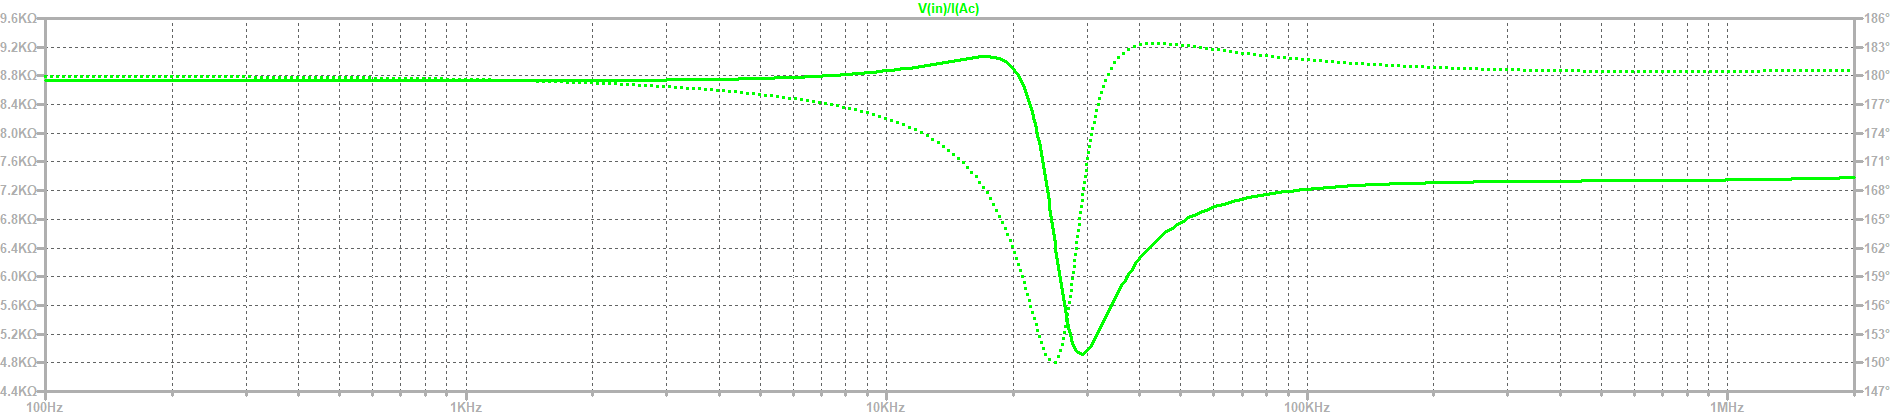
\includegraphics[width=\textwidth]{Imagenes-Ej2/ZinE1.png}
	\label{fig:graph}
	\caption{Impedancia de entrada 1er etapa.}
\end{figure}

\begin{figure}[H]
	\centering
	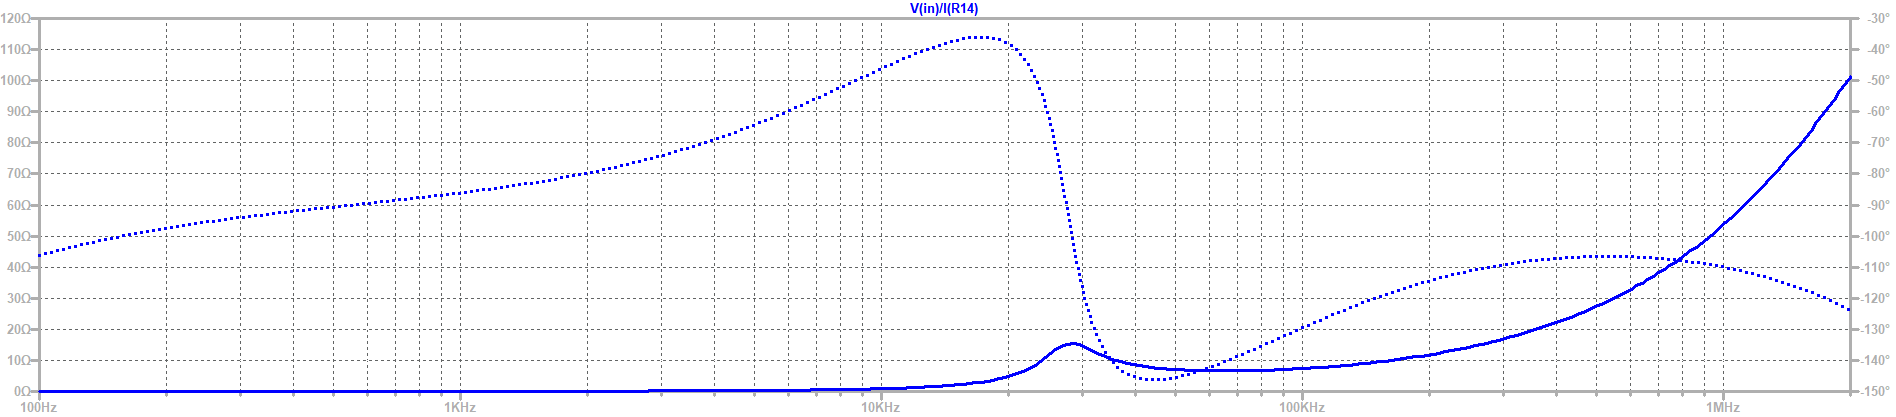
\includegraphics[width=\textwidth]{Imagenes-Ej2/ZoutE1.png}
	\label{fig:graph}
	\caption{Impedancia de salida 1er etapa.}
\end{figure}


\begin{figure}[H]
	\centering
	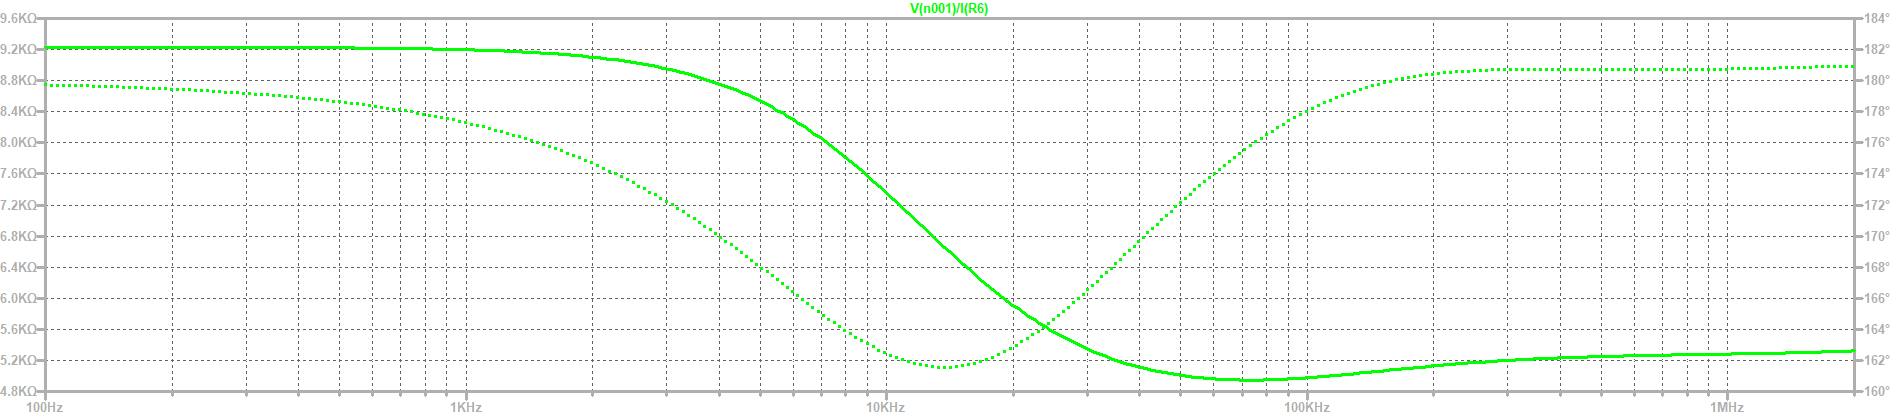
\includegraphics[width=\textwidth]{Imagenes-Ej2/ZinE2.png}
	\label{fig:graph}
	\caption{Impedancia de entrada 2da etapa.}
\end{figure}

\subsection{Respuesta en Frecuencia.}
Se realizó un análisis de Montecarlo a la respuesta en frecuencia del circuito, utilizando una tolerancia de las resistencias al 1$\%$ y capacitores al 10$\%$ obteniendo la siguiente disperción.
\begin{figure}[H]
	\centering
	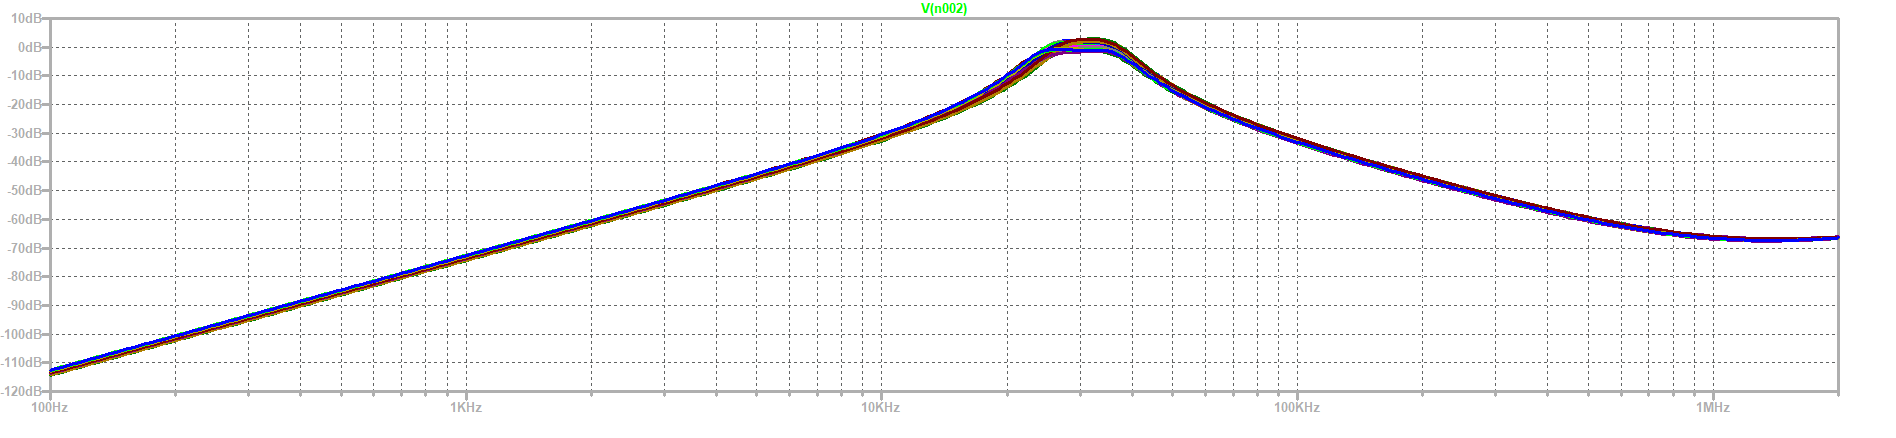
\includegraphics[width=\textwidth]{Imagenes-Ej2/mcF.png}
	\caption{Análisis de Montecarlo del filtro.}
	\label{fig:mcrauch}
\end{figure}
Se puede apreciar que la impedancia de salida de la primer etapa es bastante baja en comparación a la de entrad d e la segunda etapa, por lo tanto se dará un buen acoplamiento de impedancias y no será necesario el uso de buffers.
\subsection{Rango Dinámico.}
El rango dinámico se define como la razón de máximo y mínimo valor que puede tomar el observable de interés. Para el caso en cuestión queda definido de la siguiente manera:
\begin{align}
R_d = 20 \log_{10} \left( \frac{V_{in_{max}}}{V_{in_{min}}} \right)
\end{align}
Para definir $V_{in_{min}}$ se tuvo en cuenta la tensión mínima que se pudo distinguir respecto al piso de ruido, la cual fue de $V_{in_{min}} \approx 10mV$. Luego para definir $V_{in_{max}}$ se tuvo en cuenta la máxima tensión previo a la aparición de alinealidades, siendo estos efectos el cross-over, slew-rate y saturación del amplificador operacional, dos de estos problemas son arreglados por la elección del amplificador operacional , siendo el cross-over y el slewrate, dado a que se utilizó un TL081 el cual tiene un slew-rate elevado, y no tiene el problema del cross-over debido a su etapa de salida. Queda el problema de la saturación,es de utilidad saber que la máxima tensión de salida es $V_{sat} = Vcc-1.5 =13.5$, para encontrar el valor de tensión máximo de entrada se tomó, dada la ganancia del sistema y teniendo en cuenta la conexión entre etapas finalmente queda definido por la siguiente expresión:
\begin{align}
V_{in_{max}}=\frac{V_{sat}}{  \max(G_{E1} \cdot G_{E2} )} = 12.24V
\end{align}
Finalmente $R_d = 61.75dB$.
\subsubsection{Etapas.}
Se realizaron 2 etapas, ambas siendo el mismo tipo de celda, pero con distintos parámetros. Para cada etapa fue realizado un análisis de Montecarlo debido a la dispersión de los componentes.

\begin{figure}[H]
	\centering
	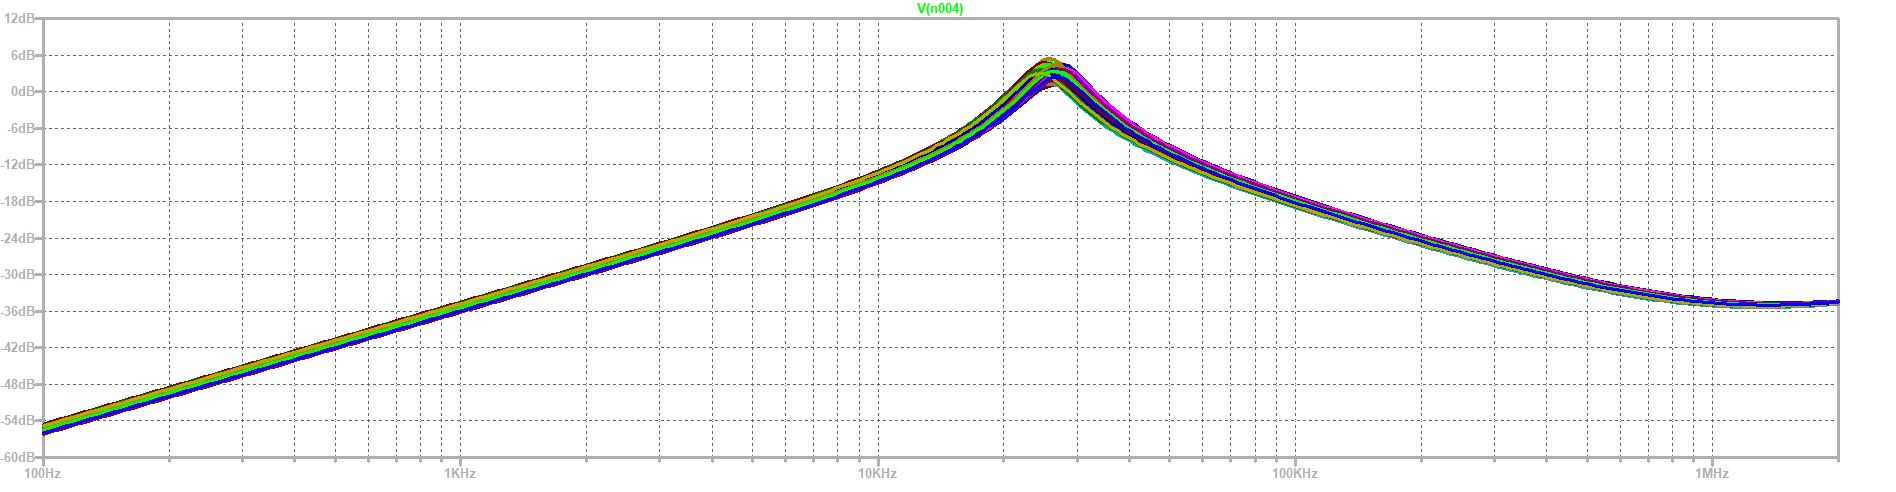
\includegraphics[width=\textwidth]{Imagenes-Ej2/mcE1.png}
	\caption{Análisis de Montecarlo primera etapa.}
	\label{fig:mcrauch}
\end{figure}

\begin{figure}[H]
	\centering
	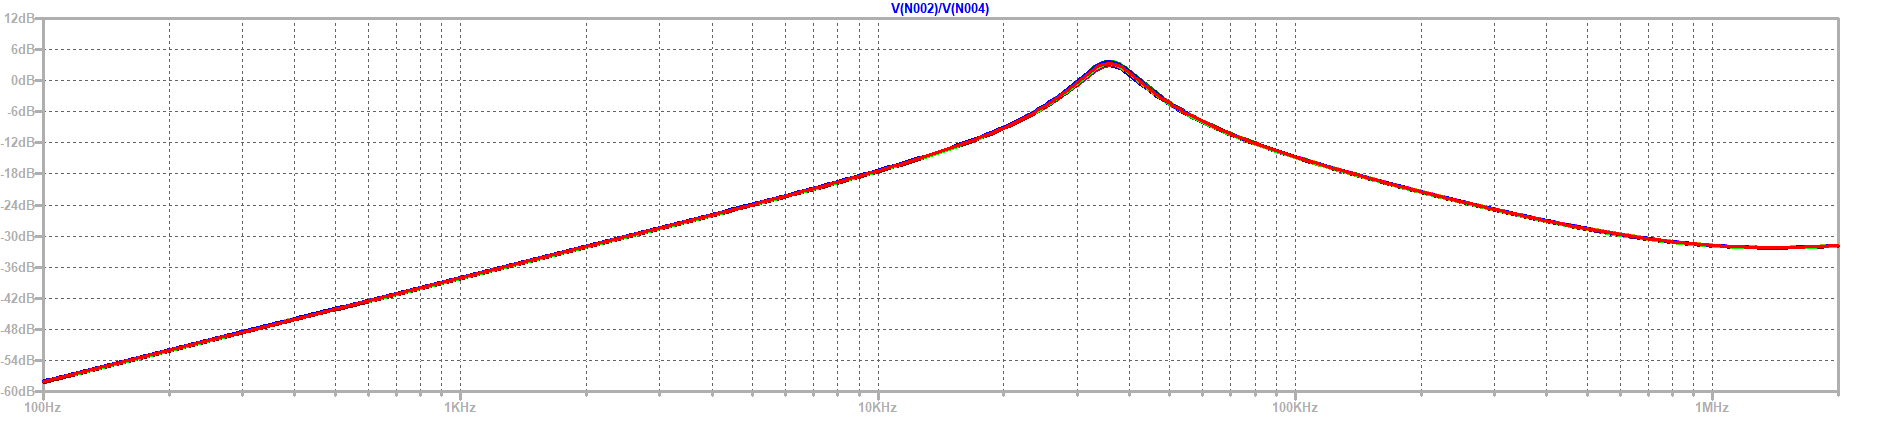
\includegraphics[width=\textwidth]{Imagenes-Ej2/mcE2.png}
	\caption{Análisis de Montecarlo segunda etapa.}
	\label{fig:mcrauch}
\end{figure}
Es notable que no existe una gran dispersión debido a los componentes en el diagrama de bode, mas allá de eso, mirando las sensibilidades se nota una gran dependencia tanto el Q y la frecuencia de corte del sistema con la resistencia R3, a continuación se verán simulaciones de montecarlo de tanto la variación de un supuesto preset sobre R3 en cada etapa y como afectan al filtro final como un todo.

Variando la resistencia R3 de la primer etapa entre 100$\Omega$ y 2k$\Omega$.  
\begin{figure}[H]
	\centering
	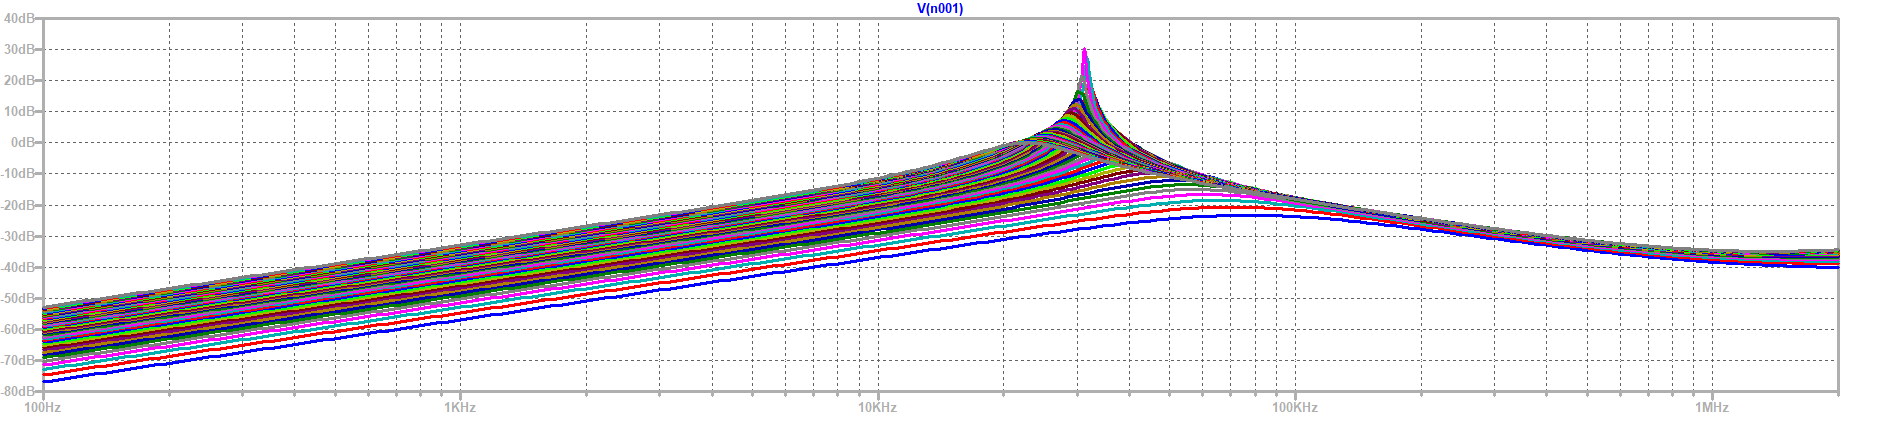
\includegraphics[width=\textwidth]{Imagenes-Ej2/presetE1.png}
	\label{fig:graph}
	\caption{Variación salida de 1er etapa al cambiar R3 de la misma.}
\end{figure}
\begin{figure}[H]
	\centering
	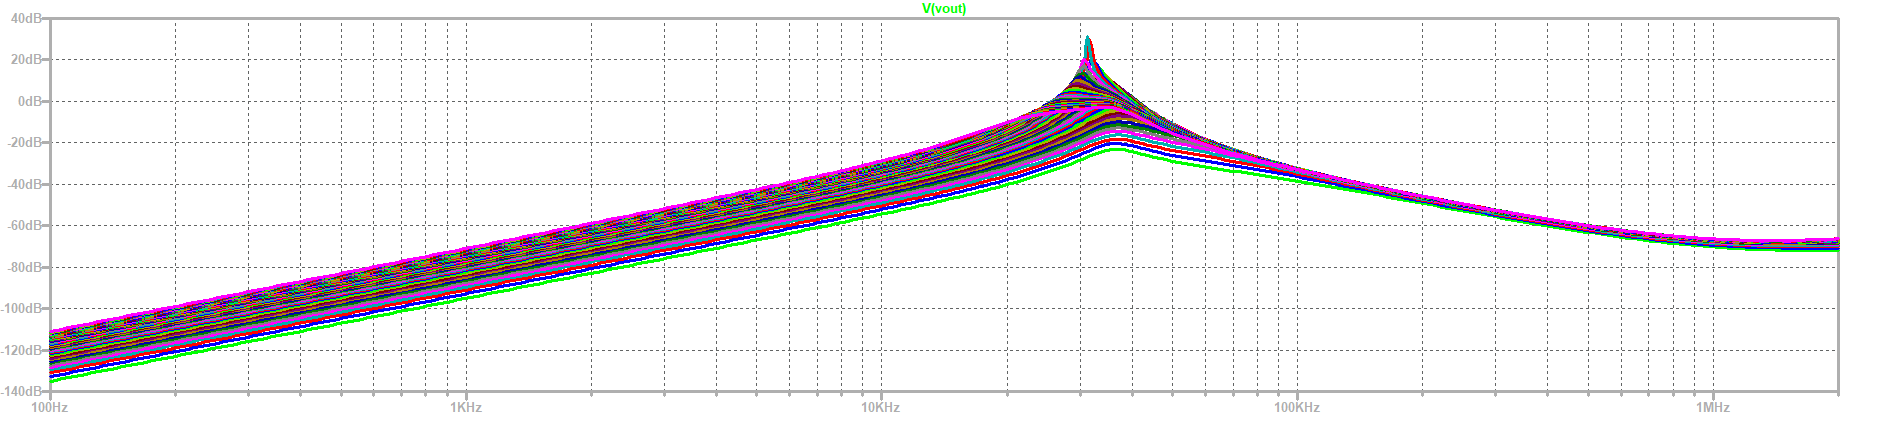
\includegraphics[width=\textwidth]{Imagenes-Ej2/presetEFE1.png}
	\label{fig:graph}
	\caption{Variación salida del filtro al cambiar R3 de la 1er etapa.}
\end{figure}
Se puede notar como se puede manipular el Q del circuito al igual que el valor de la frecuencia de corte
Luego se prosiguió por hacer el mismo análisis pero de la siguiente etapa, variando la resistencia en el mismo rango de valores.
\begin{figure}[H]
	\centering
	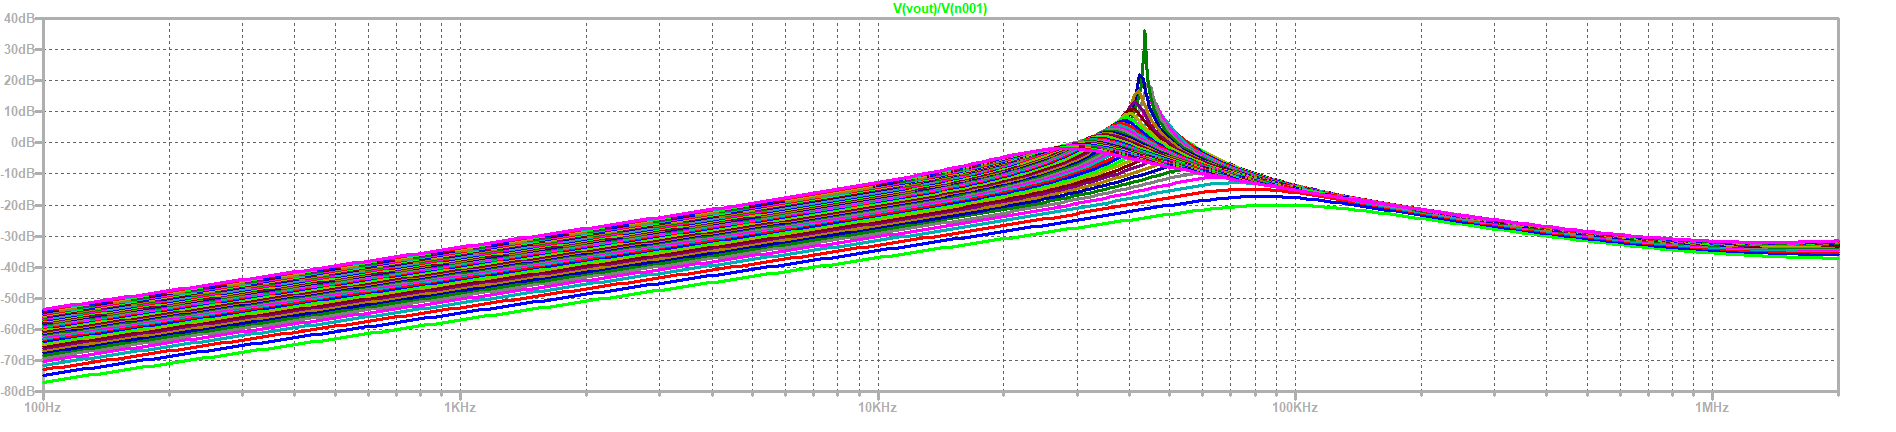
\includegraphics[width=\textwidth]{Imagenes-Ej2/presetE2.png}
	\label{fig:graph}
	\caption{Variación salida de 2da etapa al cambiar R3 de la misma.}
\end{figure}
\begin{figure}[H]
	\centering
	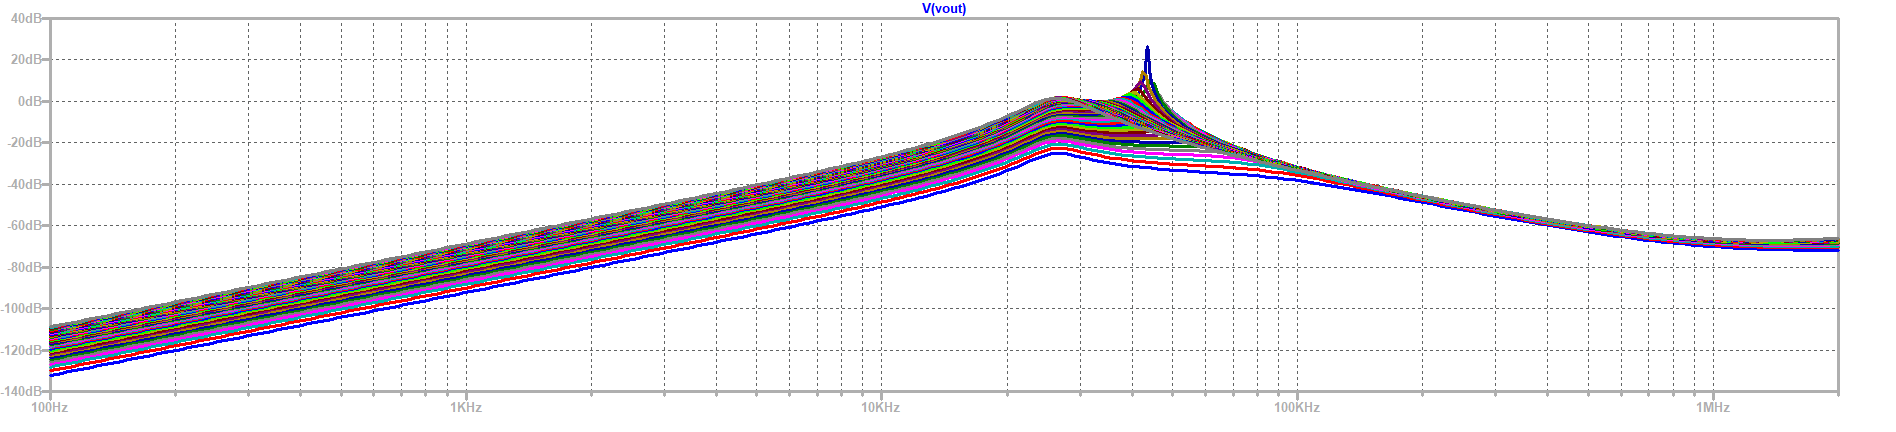
\includegraphics[width=\textwidth]{Imagenes-Ej2/presetEFE2.png}
	\label{fig:graph}
	\caption{Variación salida del filtro al cambiar R3 de la 2da etapa.}
\end{figure}
En contraparte al preset en la primer etapa, el segundo cambia de una manera mas significativa el Q mientras que es al revez con el $\omega_0$ del circuito.


Luego se realizó un histograma de la aparición de $\omega_0$ en el análisis de montecarlo.
\begin{figure}[H]
	\centering
	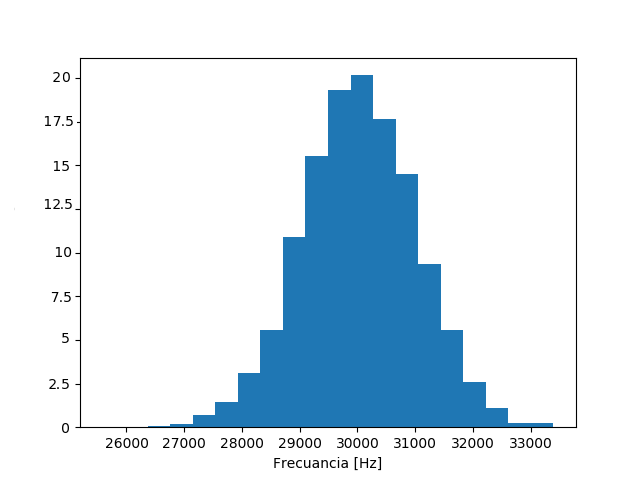
\includegraphics[width=\textwidth]{Imagenes-Ej2/histW0.png}
	\label{fig:graph}
	\caption{Histograma aparición de $\omega_0$.}
\end{figure}

\subsubsection{Filtro definitivo.}

También se midió la respuesta en frecuencia del filtro, se notó que la celda estaba amplificando de mas y no llegaba a cumplir la plantilla, por lo que se hizo una etapa de compensación de ganancia, la cual permitió que se cumplan las especificaciones. Finalmente se midió la respuesta en frecuencia obteniendo los siguientes resultados:
\begin{figure}[H]
	\centering
	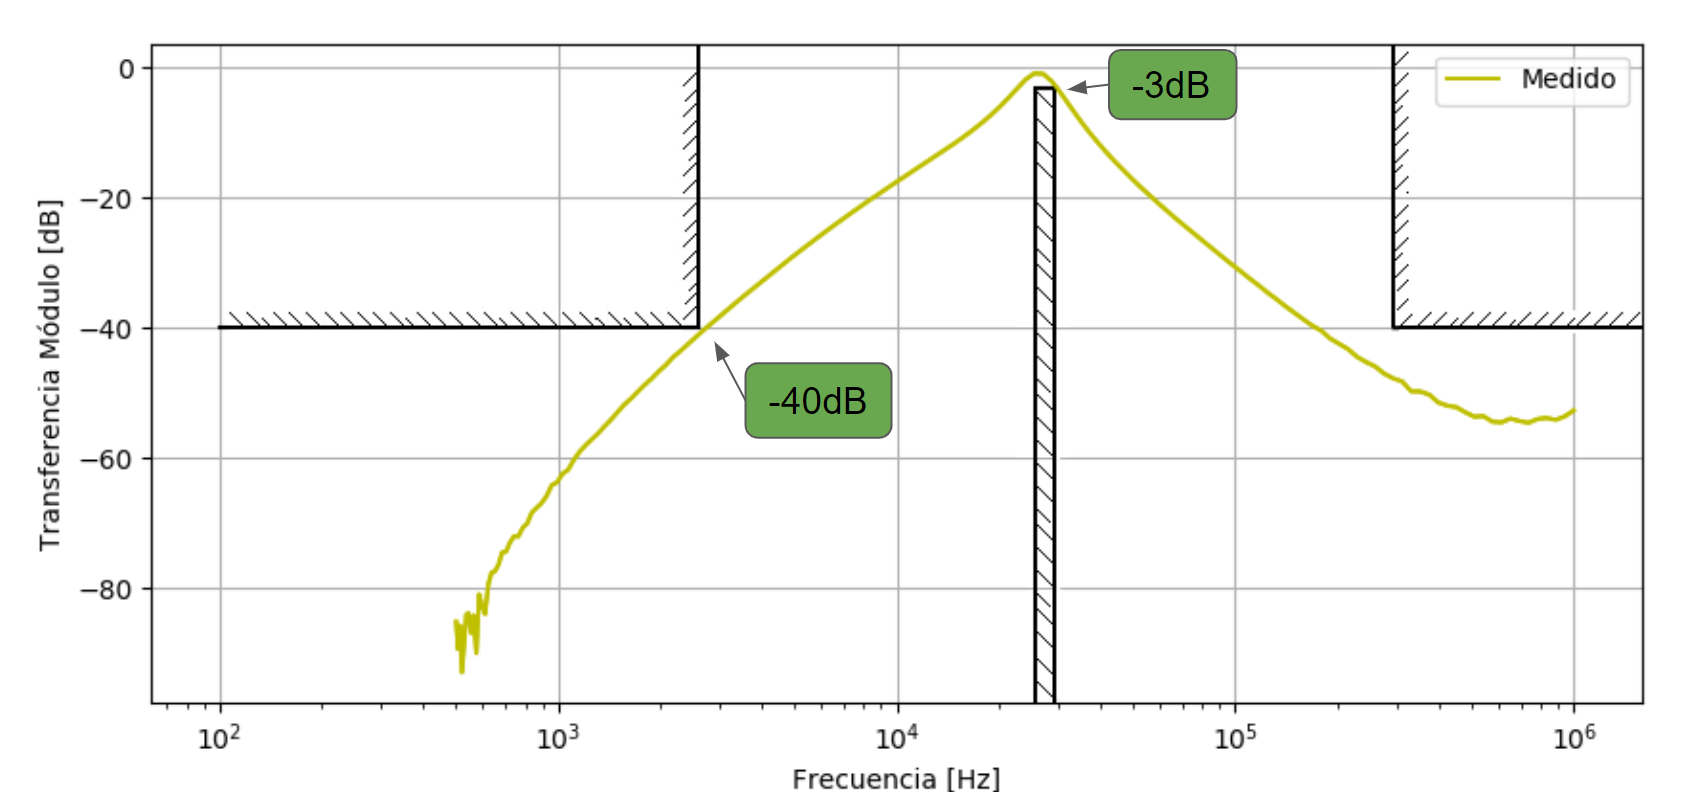
\includegraphics[width=\textwidth]{Imagenes-Ej2/BodeRauch.png}
	\label{fig:graph}
\end{figure}
\begin{figure}[H]
	\centering
	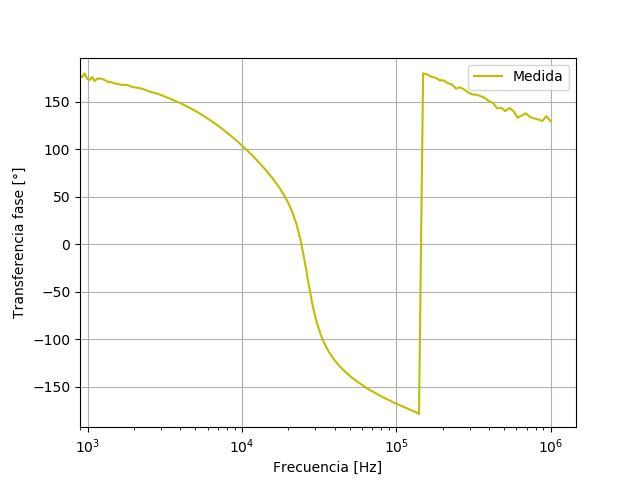
\includegraphics[width=0.7\textwidth]{Imagenes-Ej2/BodeRauchFase.png}
	\label{fig:graph}
\end{figure}
Luego se cotejó con tanto con la simulación como con el cálculo teórico.
\begin{figure}[H]
	\centering
	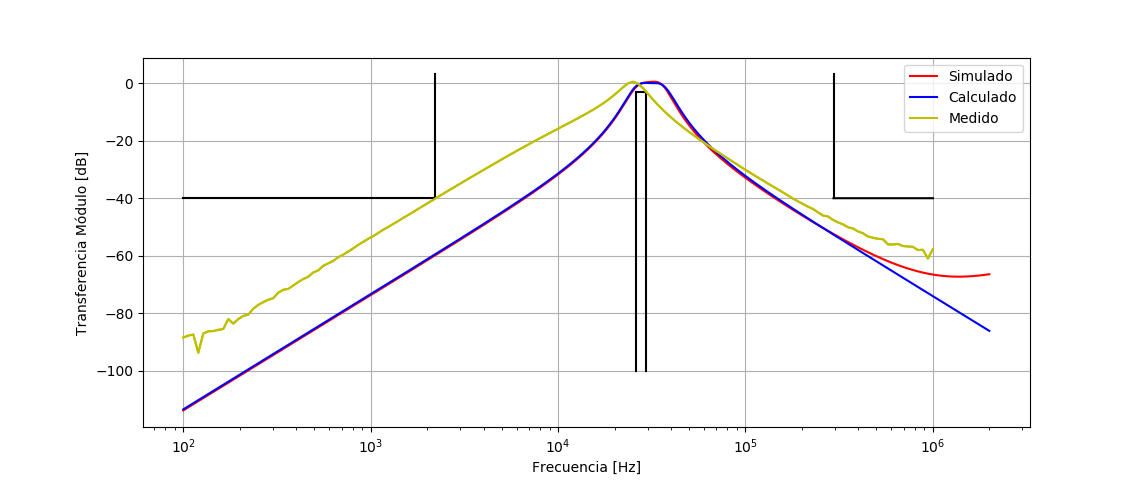
\includegraphics[width=\textwidth]{Imagenes-Ej2/BodeRauchCalcsim.png}
	\label{fig:Bodecalcsim}
\end{figure}
\begin{figure}[H]
	\centering
	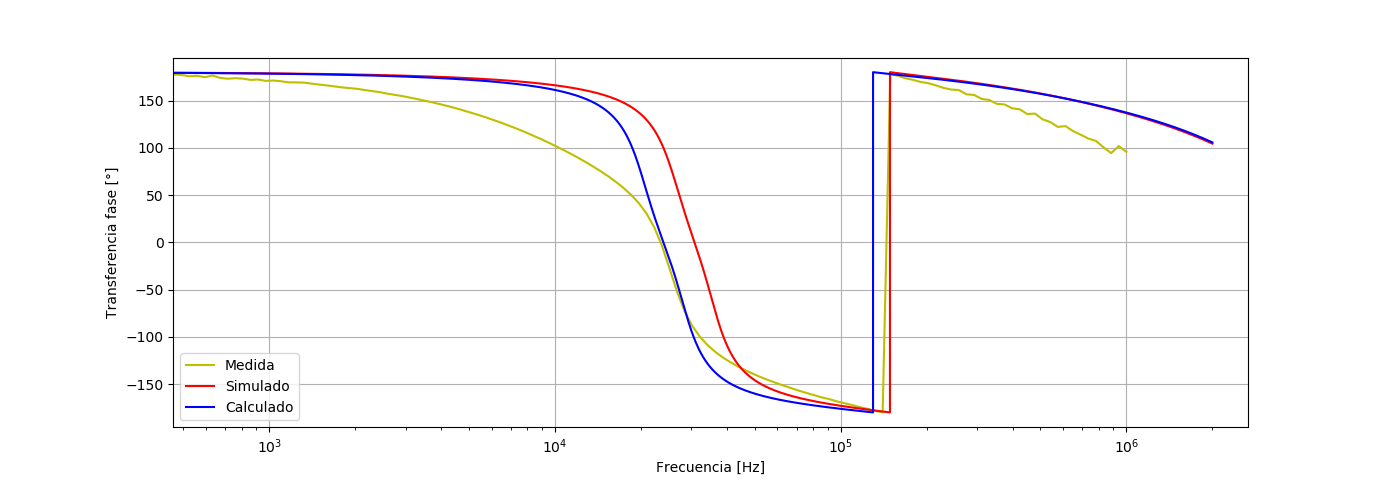
\includegraphics[width=\textwidth]{Imagenes-Ej2/BodeRauchCalcsimF.png}
	\label{fig:Bodecalcsimf}
\end{figure}
Se puede observar como el calculado y el simulado diferen ligeramente del medido, lo cual es esperado, se podría ajustar el medido mediante la utilización de presets como fue discutido previamente pero dado a que cumplía plantilla se decidió no hacerlo.
\subsection{Estabilidad}
Holi
\subsection{Conclusiones}
Se pudo realizar correctamente la implementación de un filtro pasa banda con la aproximación de chebycheff mediante celdas rauch.
Una ventaja de la celda Rauch es que permite la implementación de un filtro de segundo orden con tan solo 1 operacional, mientras que por ejemplo la celda universal utiliza 3 de ellos, también tiene el beneficio de poder sintetizar valores de Q relativamente altos gracias a su doble realimentación tanto negativa como positiva (mediante la utilización del Q enhancement), dando esta ultima una de sus desventajas que es la posibilidad de que haya una oscilación en el circuito.
También, se compensó la ganancia de manera satisfactoria al agregársele un etapa de compensación a la salida del
filtro.

%
%\begin{figure}[H]
%	\centering
%	\includegraphics[width=0.4\textwidth]{/ImagenesEjercicio3/Graph.png}
%	\label{fig:graph}
%\end{figure}

\end{document}